%
% File acl2019.tex
%
%% Based on the style files for ACL 2018, NAACL 2018/19, which were
%% Based on the style files for ACL-2015, with some improvements
%%  taken from the NAACL-2016 style
%% Based on the style files for ACL-2014, which were, in turn,
%% based on ACL-2013, ACL-2012, ACL-2011, ACL-2010, ACL-IJCNLP-2009,
%% EACL-2009, IJCNLP-2008...
%% Based on the style files for EACL 2006 by 
%%e.agirre@ehu.es or Sergi.Balari@uab.es
%% and that of ACL 08 by Joakim Nivre and Noah Smith

\documentclass[11pt,a4paper]{article}
\usepackage[hyperref]{acl2019}
\usepackage{times}
\usepackage{latexsym}
\usepackage{amsmath}
\usepackage{graphicx}
\usepackage{caption}
\usepackage{subcaption}
\DeclareMathOperator*{\argmax}{arg\,max}
\DeclareMathOperator*{\argmin}{arg\,min}

\usepackage{url}

\aclfinalcopy % Uncomment this line for the final submission
%\def\aclpaperid{***} %  Enter the acl Paper ID here

%\setlength\titlebox{5cm}
% You can expand the titlebox if you need extra space
% to show all the authors. Please do not make the titlebox
% smaller than 5cm (the original size); we will check this
% in the camera-ready version and ask you to change it back.
\newcommand\BibTeX{B\textsc{ib}\TeX}

\title{Concept Tagging for the Movie Domain}

\author{Giovanni De Toni (197814) \\
  University of Trento \\ Via Sommarive, 9, 38123 Povo,Trento TN\\
  \texttt{giovanni.detoni@studenti.unitn.it}}

\date{}

\begin{document}
\maketitle

\begin{abstract}
This work focuses on the well-known task of concept tagging sentences. This represents a relatively important challenge when doing Natural Language Processing applications since it is the starting point for more complex techniques. This report details the realization of an SLU module for concept tagging on the movie domain. It shows also the performance obtained and the results over various techniques.
\end{abstract}

\section{Introduction}
One of the first and most important of any NLP task is to analyze a given phrase to understand its underlying meaning. More specifically, we want to find the most likely interpretation which maps the phrase to given concepts. For instance, imagine we are using a vocal application to order something to eat (e.g., "I would like a tortel di patate delivered at Piazza Trento 1, please"). For a machine to understand correctly what we want, firstly it needs to convert our utterances to a word representation, secondly, it needs to assign a concept to each of the words it heard (e.g., "tortel di patate" equals to an hypothetical "FOOD" concept and "Piazza Trento 1" equals to the "DELIVERY ADDRESS").
This basic operation is of utmost importance for all the application which can be built upon this. For instance, the quality of your food assistant is dependent on the quality of this concept tagger. Imagine what could happen if the machine were to swap the delivery address with the requested food!.  
The scope of this project is to provide a simple concept-tagger by developing a WSTF (Weighted Finite-State Transducer) applied to the movie domain.
The report is structured as follow: the first section defines more formally the problem statement, then we proceed with an analysis of the given dataset and with the description of the models employed. Ultimately, we discuss the obtained results while underlying their strengths and limitations.
 

\section{Problem Statement}
Given a sequence of tokens $<t_1, \ldots, t_n>$ and given a pool of concepts $<c_1, \ldots, c_m>$, we want to find the most likely assignment $<t_i, c_i>$ such that it maximizes the following probability:
\begin{equation}
c_1, \ldots, c_n = \argmax_{c_1, \ldots, c_n} P (c_1, \ldots, c_n | t_1, \ldots, t_n)
\label{frm:argmax}
\end{equation}
The previous formula can be made easier to compute thanks to the Markov assumption. The probability of the $i$-th concept $c_i$ depends only on the $(i-1)$-th concept $c_{i-1}$ and the probability of the $i$-th token $t_i$ depends only on the $i$-th concept $c_i$. We can estimate the various parameter by Maximum Likelihood (MLE):
\begin{equation}
c_1, \ldots, c_n = \argmax_{c_1, \ldots, c_n} P(t_i|c_i)P(c_i| c_{i-1})
\label{frm:argmax-markov-assumption}
\end{equation}
In the previous formula, $P(t_i|c_i) = \frac{C(c_i, t_i)}{C(c_i)}$ and $P(c_i|c_{i-1}) = \frac{C(c_{i-1}, c_i)}{C(c_i)}$ (where $C(x)$ counts the occurrences of $x$ inside the given dataset). 

\begin{table*}
    \begin{subtable}{.5\linewidth}
		\centering
\begin{tabular}{|l|l|}
\hline
\multicolumn{2}{|l|}{\textbf{NL2SparQL4NLU.trai.conll.txt}} \\ \hline
\textit{\# of lines}									& 24791 \\ \hline
\textit{\# of sentences}                             & 3338 \\ \hline
\textit{\# of unique tokens}                         & 1728 \\ \hline
\textit{\# of unique concepts (without the prefix)}  & 24   \\ \hline
\end{tabular}
\caption{Train dataset.}
\end{subtable}%	
\begin{subtable}{.5\linewidth}
\centering
\begin{tabular}{|l|l|}
\hline
\multicolumn{2}{|l|}{\textbf{NL2SparQL4NLU.test.conll.txt}} \\ \hline
\textit{\# of lines}									& 8201 \\ \hline
\textit{\# of sentences}                             & 1084 \\ \hline
\textit{\# of unique tokens}                         & 1039 \\ \hline
\textit{\# of unique concepts (without the prefix)}  & 23   \\ \hline
\end{tabular}
\caption{Test dataset.}
\end{subtable}
\caption{Description of the content of the dataset used.}
\label{tab:test-dataset-description}
\end{table*} 

\section{Data Analysis}

The dataset used is called NL2SparQL4NLU\footnote{https://github.com/esrel/NL2SparQL4NLU} \citep{Chen2014DerivingLR, gobbi2018concept}. It contains several english sentences related to the movie domain. This work used only the ``*.conll.txt" files. More specifically, one for training the language model and one for testing it. Each file is written using the token-per-line CONLL format with tokens and NLU concept tags. Table \ref{tab:test-dataset-description} provides a general description of the two files. The average length of the sentences is around 6.42 and 6.52 for the train and test dataset respectively. The OOV rate for the tokens between the train and the test datasets is around $0.24\%$.


Figure \ref{fig:concept-distribution} shows the distribution of the various concepts. There are 43 concepts tag in the dataset (with the IOB tags) and 23 without the prefix. We noted that the ``\textit{O}" concept represent the $70\%$ of the dataset, which pose a big problem for the next tagging procedure. The concepts graph do not show the "O" concept to make it easier to visualize the distribution of the other concepts. It is possible to see how the \textit{movie.name} concept is one of the most common, followed by \textit{actor.name} and \textit{director.name}.

Both train and test set contains concepts which are not present in the other dataset (and viceversa). The train dataset contains \textit{person.nationality} (2 occurrences) and \textit{movie.description} (2 occurrences) which are not present in the test set. The test dataset contains the concept \textit{movie.type} which is missing from the train dataset (4 occurrences). These again could cause mistagging issues and therefore lower the final performance of the SLU model. 
As a final note, there are also
some tokens which are the results of mispelling (e.g., ``dispaly", ``Scorcese") which therefore could lead to other tagging errors.


\section{Models}

\begin{figure}[b!]
\centering
	\includegraphics[width=1\linewidth]{img/entity}
	\caption{Example of entity recognition. For instance, the ``\textit{ed harris}" tokens were recognized as a PERSON while ``\textit{thirteen}" was recognized as number. Therefore, the ``\textit{ed harris}" tokens will be replaced by the entity ``PERSON"}
	\label{fig:entity-recognition}
\end{figure}

In this work we devised and evaluated two separated SLU models. 
The first SLU model was trained by using directly 
the dataset provided (without modifications). It 
implements Formula \ref{frm:argmax-markov-assumption}. 
This first model was used as the baseline. The second 
model uses entity recognition (ER) tools which convert 
certain token(s) to an entity definition prior training 
the complete language model. See Figure \ref{fig:entity-recognition} for an example of entity recognition. These 
entity definitions replace the previous tokens. We choose two external libraries which provides two pre-trained ER classifier: NLTK \cite{nltk} and spaCy \cite{spacy2}. 
We performed these improvements to mitigate some ambiguity and variability issues which are presents in the dataset. 
More specifically, some tokens refer to the same entity 
and the same concept while they may have different values 
(e.g., \textit{nick fury} and \textit{robin} are both 
persons (entity) and character names (concept), even if 
they have different tokens). 
As the analysis showed us, the majority of the dataset 
concepts  are equal to ``\textit{O}" which is not 
informative enough. A possible solution is to substitute 
each occurrences of the  ``\textit{O}" concept with 
another value, such to increase the final performances.
We tried three possibile substitution policies. We used: 
directly \textbf{the token}, the \textbf{token's stem} and the \textbf{token's lemma}. 


\begin{figure*}
	\begin{subfigure}[b]{0.5\linewidth}
		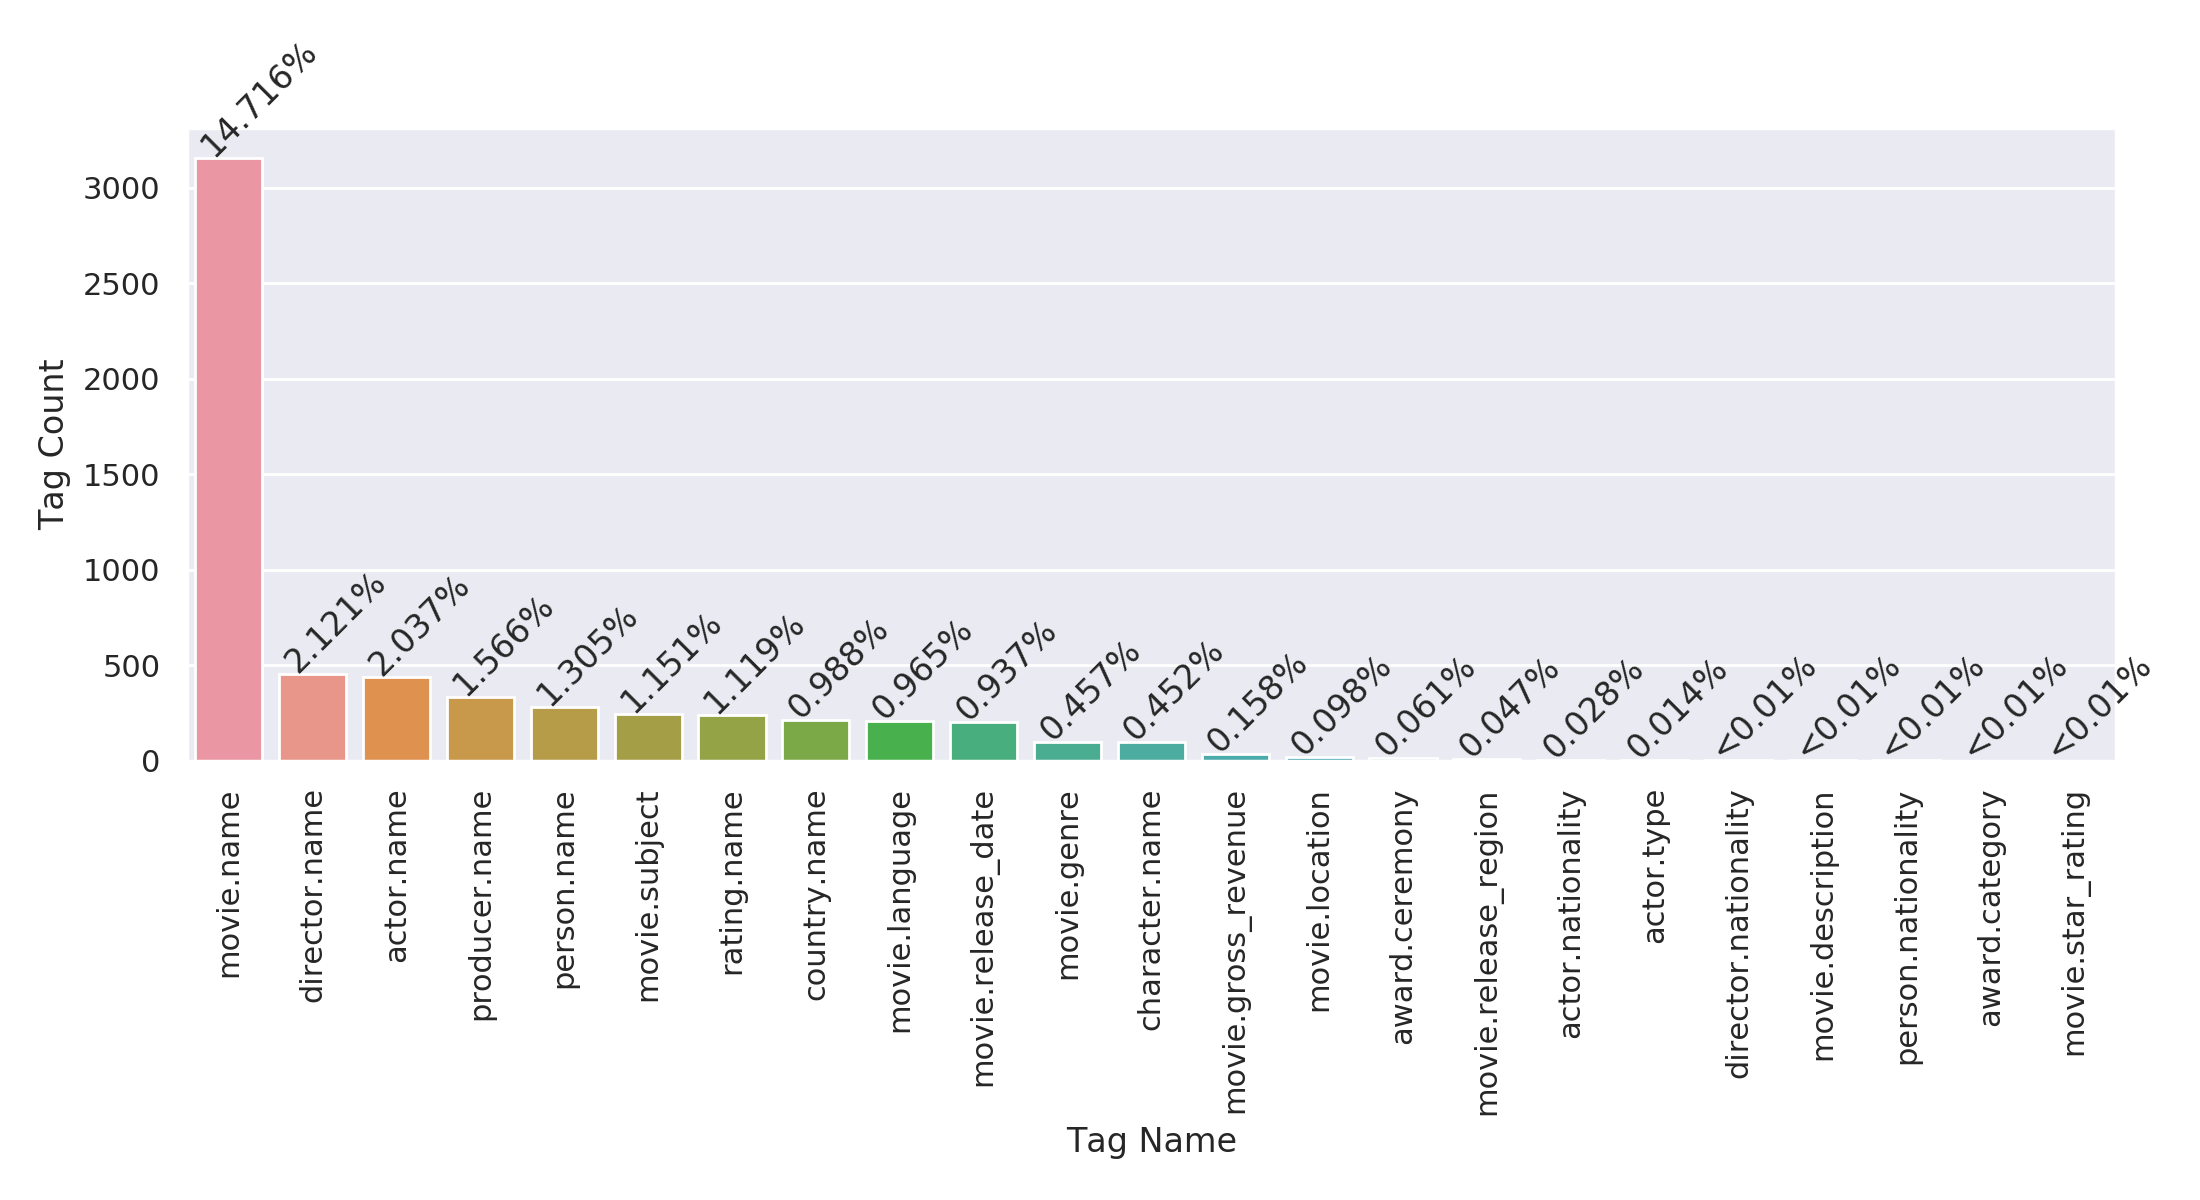
\includegraphics[width=\linewidth]{img/train-concepts-distribution}
		\caption{Train dataset.}
	\end{subfigure}
	\begin{subfigure}[b]{0.5\linewidth}
	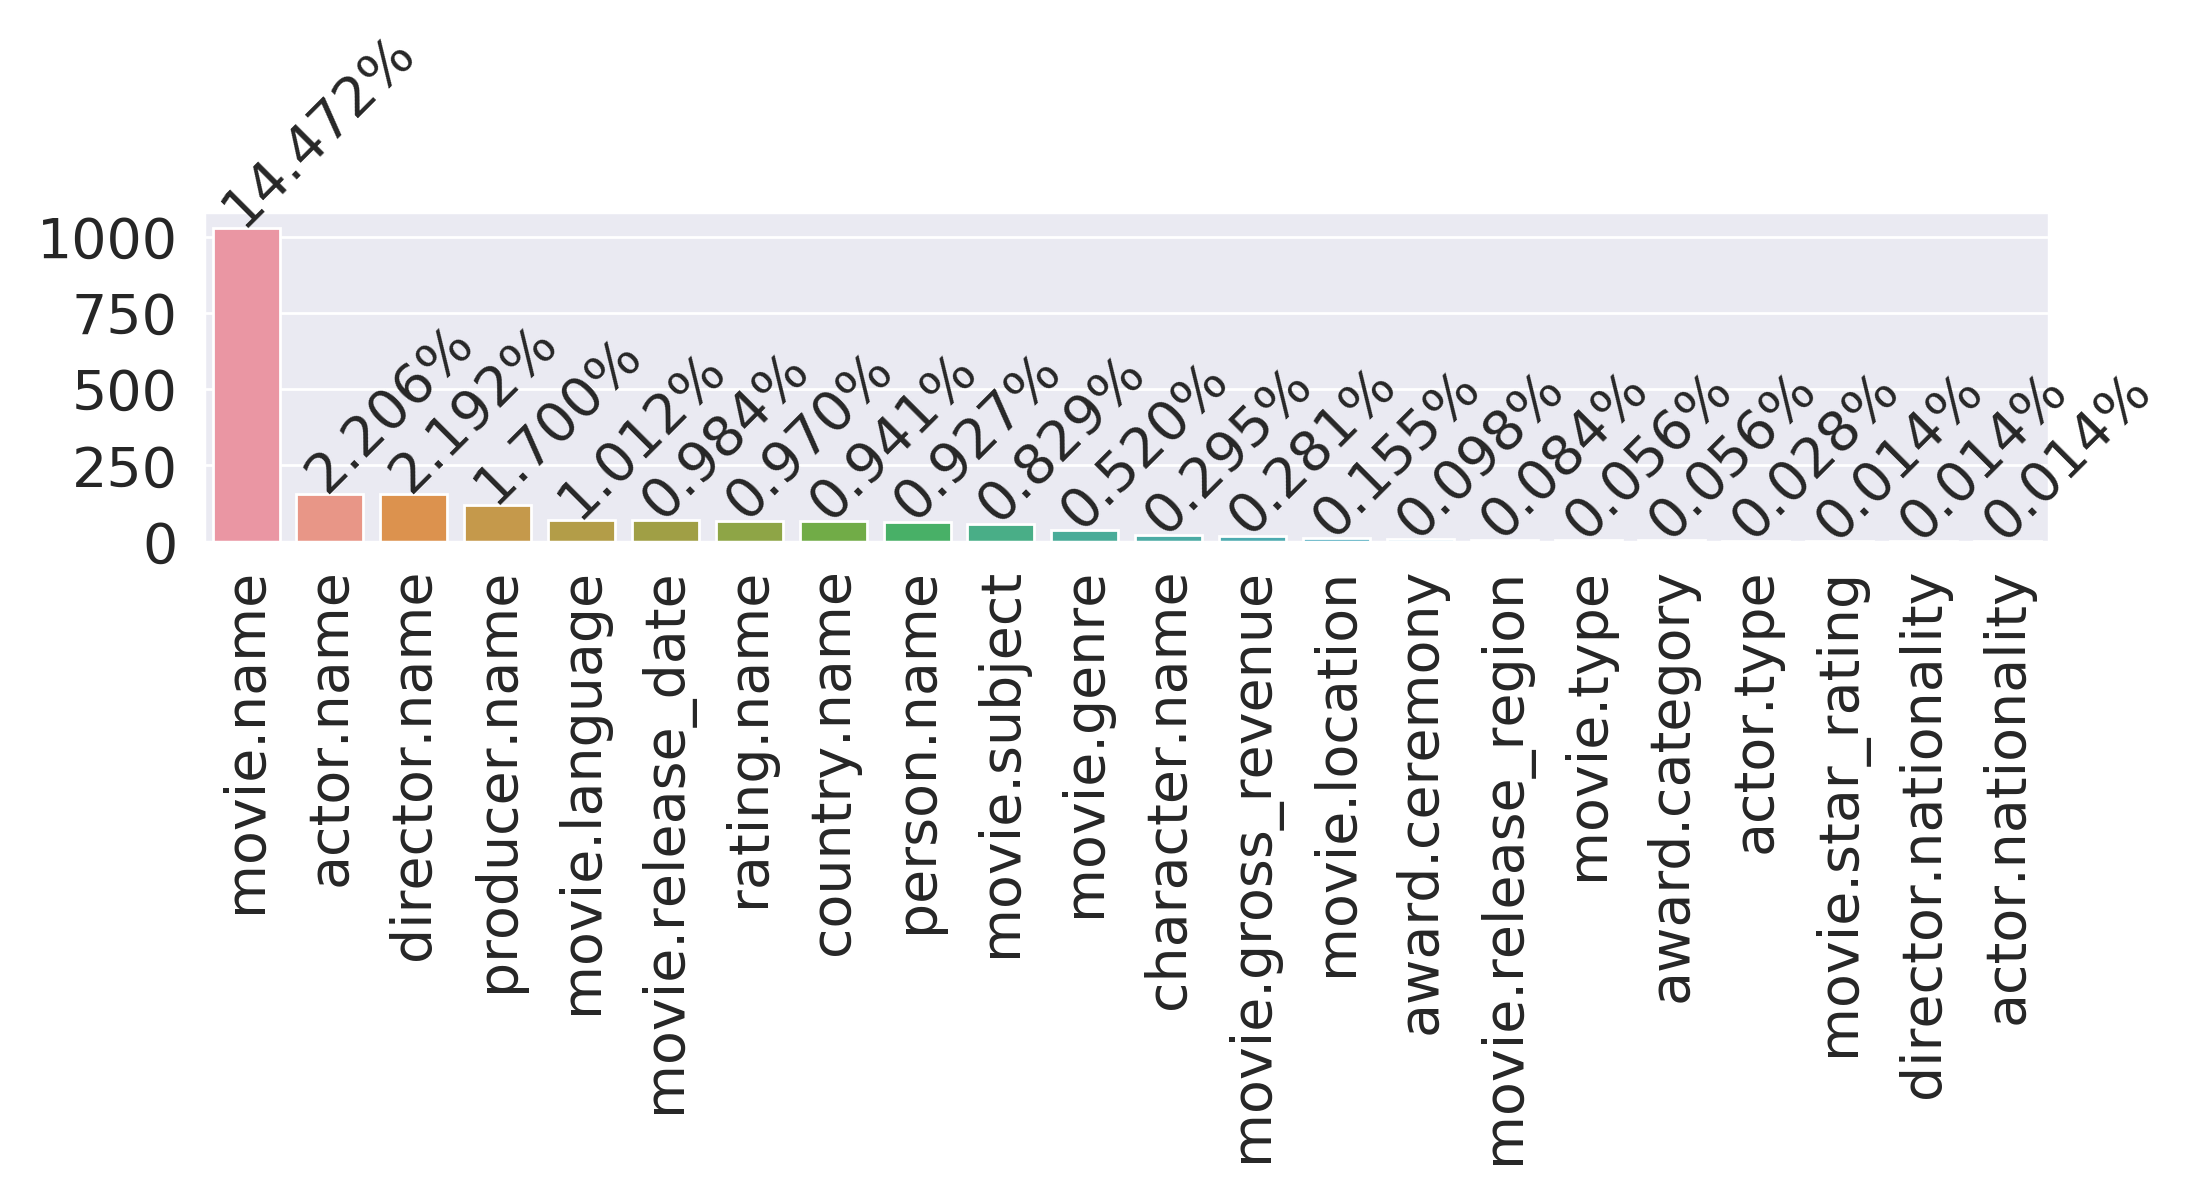
\includegraphics[width=\textwidth]{img/test-concepts-distribution}
	\caption{Test dataset.}
	\end{subfigure}
	\caption{Distributions of the various concepts in the train and test datasets. The \textit{O} concept was removed to make it easier to understand the weight of the other concepts.}
	\label{fig:concept-distribution}
\end{figure*}

\subsection{Spoken Language Understanding Pipeline}
The entire SLU pipeline of both models is composed of two main components:
\subsubsection{Concept Tagger (WFST)}
It is a transducer which encodes the probability $P(t_i|c_i) = \frac{C(c_i, t_i)}{C(c_i)}$. The probability (score) is the weigth given to the transition from the given token to the concept. In order to solve possible numerical stability issue, the negative log was applied to the probability. Therefore, the weigth assigned to the transitions is computed by using $-log(P(t_i|c_i))$. An additional token called $<$\textit{unk}$>$ was added to the transducer to account for unknown words (namely, tokens which are present in the test dataset, but not in the train dataset). Moreover, for each of the possible concepts $c_i$, a transition $<$\textit{unk}$>$:$c_i$ was added with a score of $\frac{1}{\#concepts}$ (this means that each unknown token has an equal probability of ``representing" each concepts). 
\begin{figure}[b!]
	\centering
	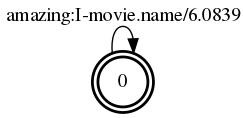
\includegraphics[width=0.5\linewidth]{img/pos-tagger}
	\caption{Example of a possible transducer in which the token \textit{amazing} is mapped to the concept \textit{I-movie.name} with an associated transition score.}
\end{figure}

\subsection{Language Model (LM)}
It is a transducer which encodes the probability $P(c_i|c_{i-1}) = \frac{C(c_{i-1}, c_i)}{C(c_i)}$, which mean finding a concept $c_i$ conditioned on having seen concept $c_{i-1}$. 

\subsection{Final SLU Model}

The previous components needs to be composed together with the sentence we want to tag to be used.
\begin{equation}
\lambda_{CT} = \lambda_{sentence} \circ \lambda_{WFST} \circ \lambda_{LM}
\end{equation}
Then, we need to find the path which minimize the cost within the final transducer (since we are using $-log()$ to compute the weigths, minimizing the path cost is the equivalent of maximizing the probability of that tagging sequence). This final operation corresponds to computing the equation shown in Formula \ref{frm:argmax-markov-assumption}.

\section{Experiments}

Several experiments were run to assess the quality of 
the concept taggers. As a metric, we tried to find the solution which maximize the \textit{F1-score} over the test set. For each provided solution, we perfomed an extensive hyperparameter search by trying several \textbf{smoothing techniques}, \textbf{ngram sizes} and \textbf{pruning frequencies}. Each solution was evaluated by using k-fold cross-validation ($k=5$) and the best result was then recorded. Firstly, we evaluated the SLU model based directly on the given dataset without any further improvements. The best combination was then used as a baseline. Secondly, we evaluated the ER SLU model. The results are summarized in Table \ref{tab:eval-resuts}.

The code employed for the project is publicy available on Github\footnote{https://github.com/geektoni/concept\_tagging\_NLP}. The script were written using Python 3.6 and bash. OpenFST \cite{openfst} and OpenNGRAM \cite{opengrm} libraries were used to build the WFST and the language model. The spaCy\footnote{https://spacy.io/} and NLTK\footnote{https://www.nltk.org/} libraries were used to perform entity recognition.
The experiments were run on a 8th-core Intel i7 CPU with 16GB of RAM. 

\section{Results}

\begin{table*}[h!]
\centering
\caption{Evaluation results}
\label{tab:eval-resuts}
\begin{tabular}{llllll}
\hline
\textbf{ngram size} & \textbf{smoothing used} & \textbf{pruning} & \textbf{replace O} & \textbf{k-fold F1 score} & \textbf{k-fold F1 score (ER)} \\ \hline
4 & kneser\_ney & 5 & keep & 75.04 & 74.41 \\
4 & kneser\_ney & 5 & lemma & 83.45 & 83.27 \\
4 & kneser\_ney & 5 & stem & 83.61 & 83.47 \\
4 & kneser\_ney & 5 & word & 83.73 & 83.49 \\
4 & witten\_bell & 5 & keep & 75.32 & 74.53 \\
4 & witten\_bell & 5 & lemma & 83.29 & 83.43 \\
4 & witten\_bell & 5 & stem & 83.38 & 83.55 \\
4 & witten\_bell & 5 & word & 83.36 & 83.40 \\ \hline
\end{tabular}
\end{table*}

Despite our efforts, it seems that the ER SLU model do not add any improvements to the previous solutions. As we can see from Table X, the ER models are not even able to even reach the baseline performances in all of the various experiments we did. The best results were obtained using XXX...

This performace decreases happens for many different reasons. First of all, the spaCy entity resolution tool is not very precise. It was trained on the OntoNotes dataset [add citation] which is a general source for annotated text. It is not specific for the movie domain. Therefore, the label used are quite general (e.g., PERSON instead of ACTOR or DIRECTOR). For example, this caused some wrong entity recognition tagging (e.g., apollo 13 is the title of a film, but just 13 was recognized as a CARDINAL entity, while both the tokens should have had recognized).
Secondly, the original dataset has some issues regarding its concepts definition. Some of the them are very similar and they represent the same entity in the end. For instance, movie.location and move.country indicates states and it can be difficult to differentiate between them. Therefore, it happens that some tokens are tagged as movie.location instead of movie.country.  


\bibliography{acl2019}
\bibliographystyle{acl_natbib}

\end{document}
